\chapter{Detector Characterization}
The last step of manufacturing is to test the electrical properties of the detector and evaluate whether it is functioning properly or not.
Several properties must be analyzed in order to determine the quality of the detector; the first of which is leakage current.
In order for the detector to work properly, it must function as a basic capacitor.
If current can flow while the detector has applied voltage, then the amorphous germanium layer is not properly blocking holes and electrons which means the detector will not function.
Thus, a measure of leakage current is a necessary initial step to analyze if the detector will work at all.

If the leakage current is tested and determined to be of an acceptable level (on the order of a few picoamps or less), testing can proceed.
The next property measured is the detector capacitance.
This measurement is made using an injected pulsar and can also determine the depletion voltage of the detector.
The detector capacitance and depletion voltage can also give an accurate measurement for the impurity concentration of the germanium.
Finally the detector spectrum is measured using several radioactive sources such as cobalt 60 and cesium 137.
From this spectrum, the energy resolution of the detector can be determined and thus the overall quality.

All of these measurement must be taken while the detector is at cryogenic temperatures as described in chapter 2.
They also require the integration of several pieces of electronics that must be easily interchanged to make the different measurements.
The cryostat used at USD is shown in Figure \ref{fig:cryostat-whole}.
In the figure, the black cords coming into the base on the right and left side are a mix of high voltage and signal cables.
The flex tube coming into the middle is a vacuum tube.
The large black cylinder on top is the chicken feeder style liquid nitrogen dewar.
The metal cylinder at the base is where the detector sits.
\begin{figure}[htpb]
\centering
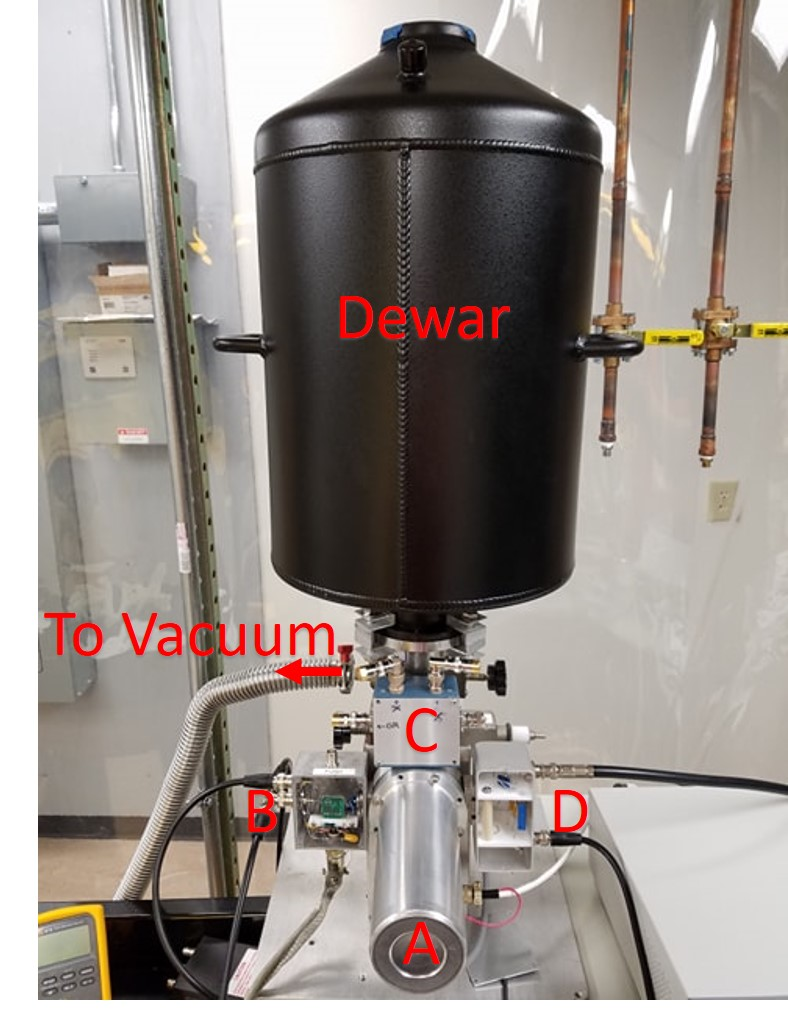
\includegraphics[width=\textwidth]{cryostat-whole}
\caption{Cryostat system used for detector calibration.}
\label{fig:cryostat-whole}
\end{figure}


\begin{figure}[htpb]
\centering
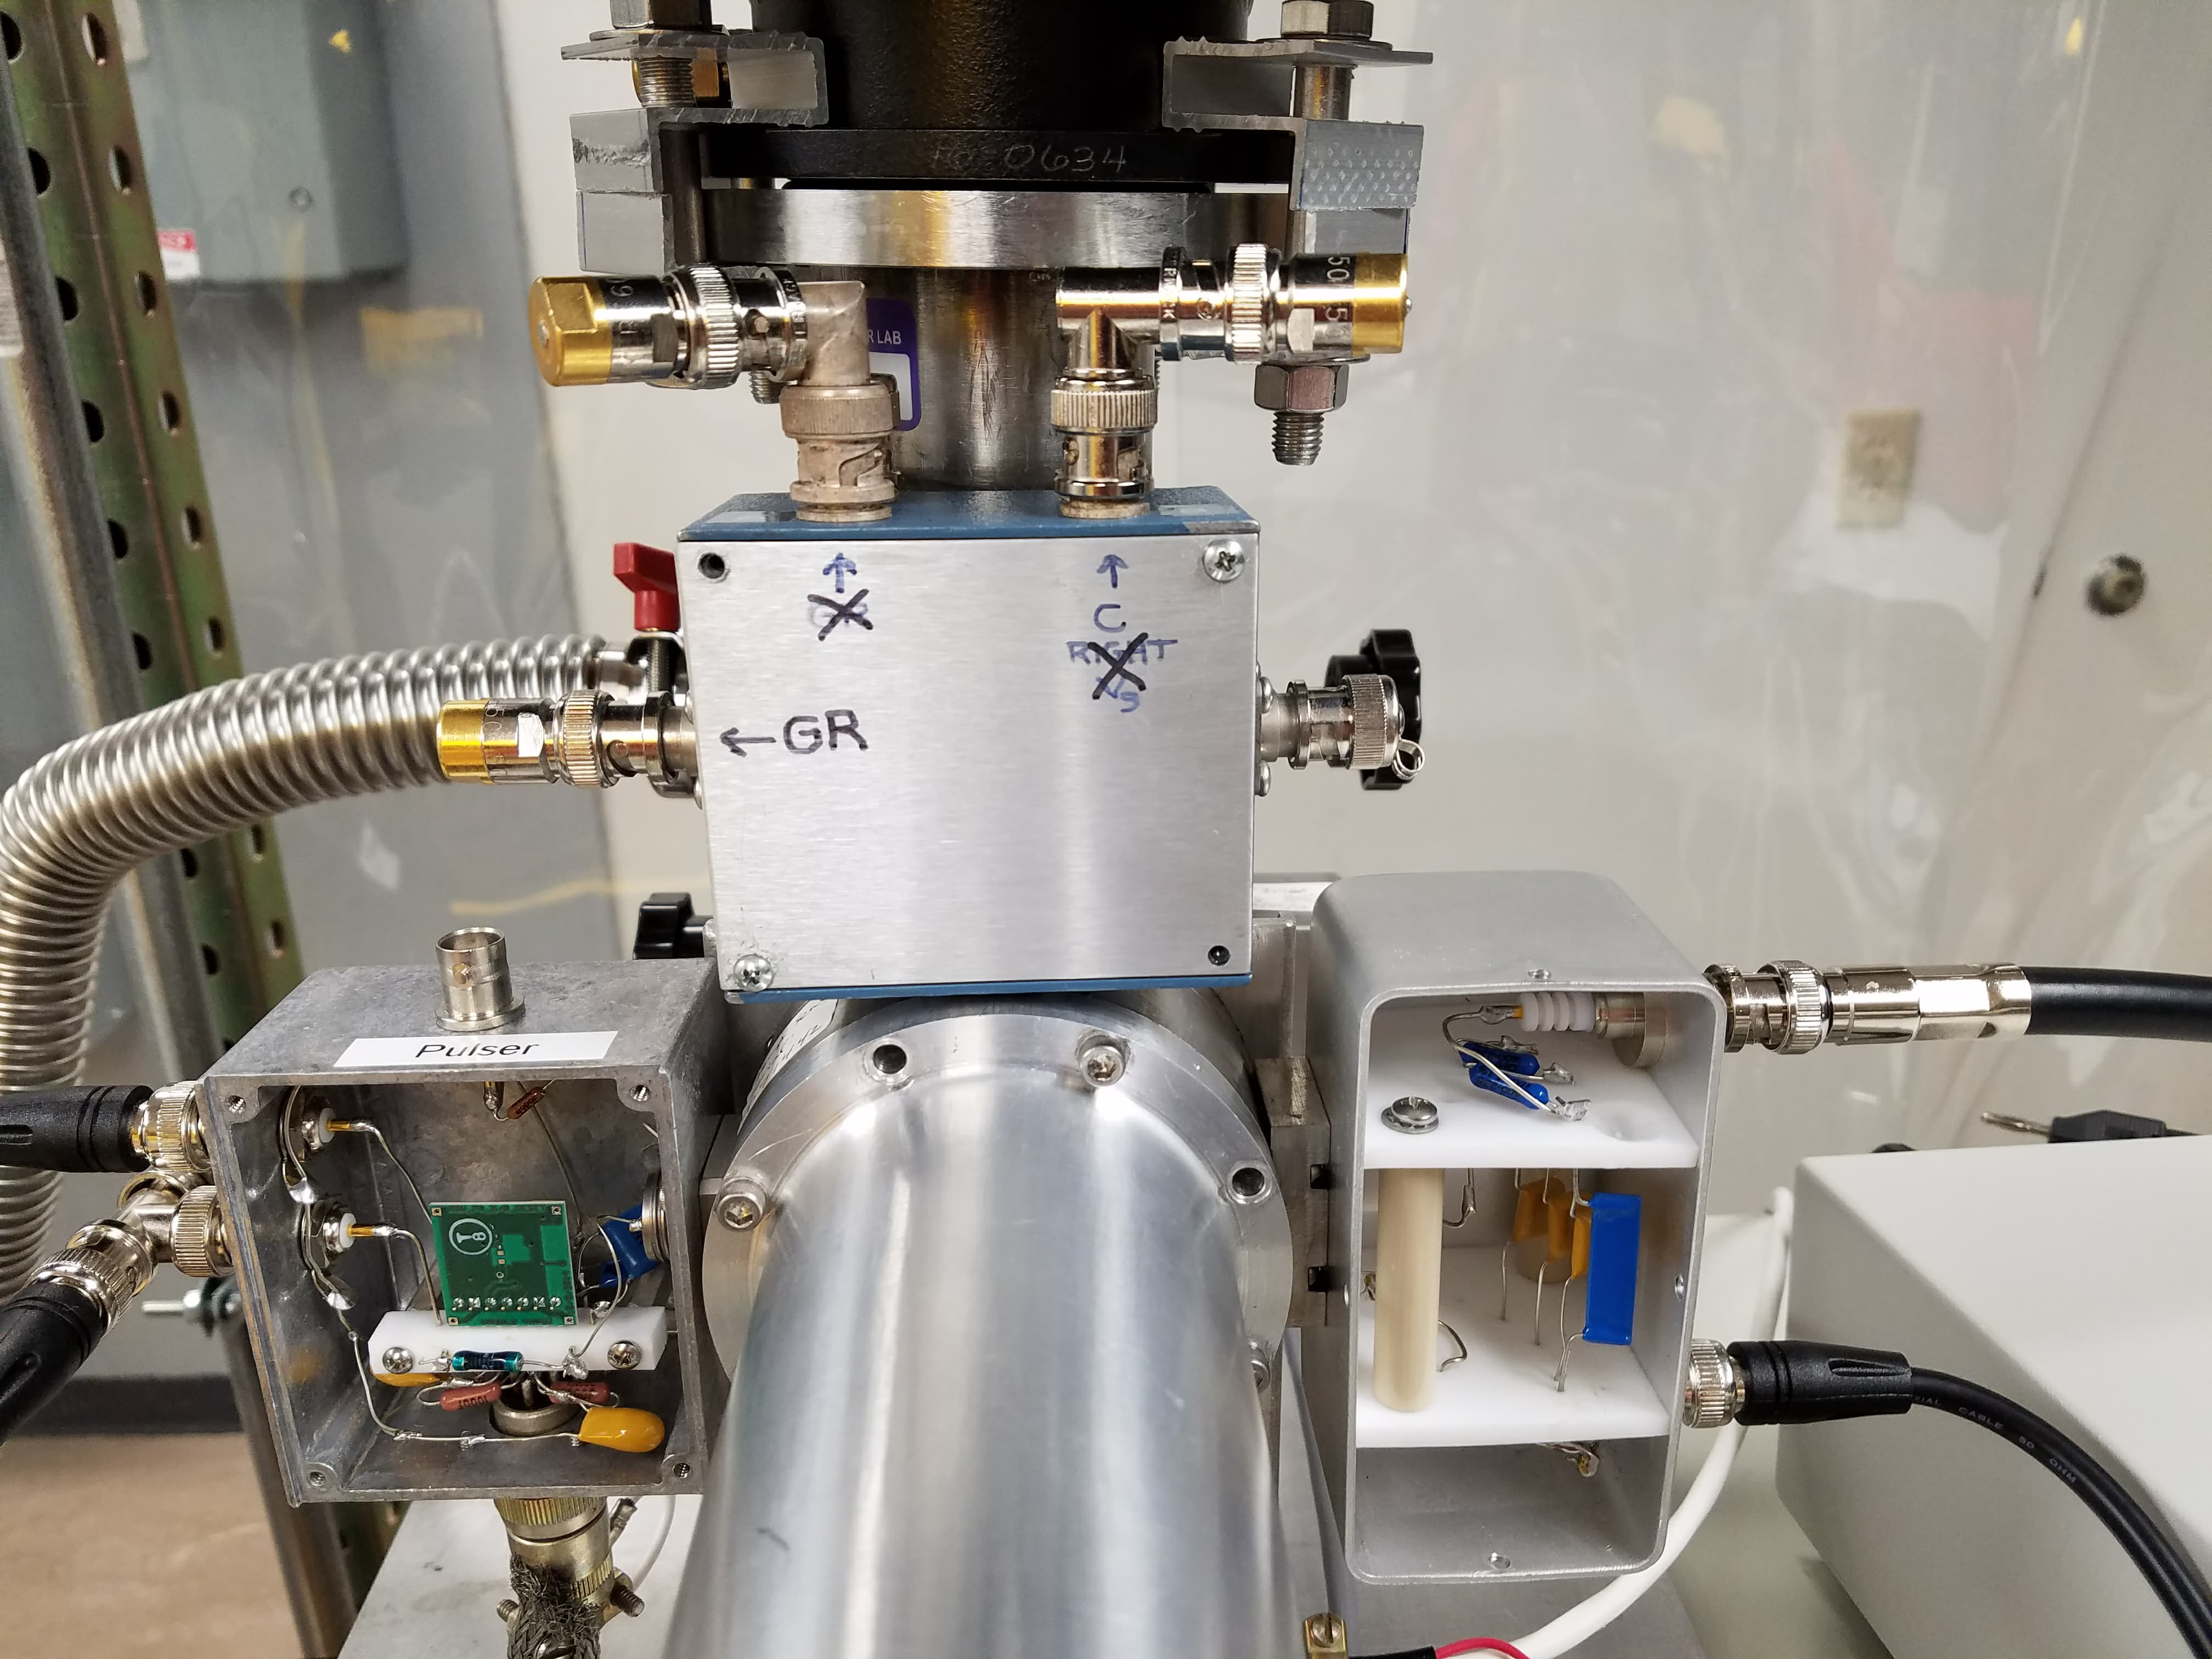
\includegraphics[width=0.7\textwidth]{inputs}
\caption{Zoomed in view of the electrical inputs and circuitry}
\label{fig:inputs}
\end{figure}

\begin{figure}[htpb]
\centering
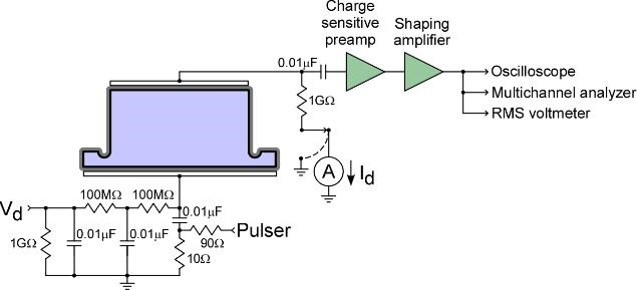
\includegraphics[width=0.7\textwidth]{outline}
\caption{Simple circuit diagram of the germanium detector electronics}
\label{fig:outline}
\end{figure}

\begin{figure}[htpb]
\centering
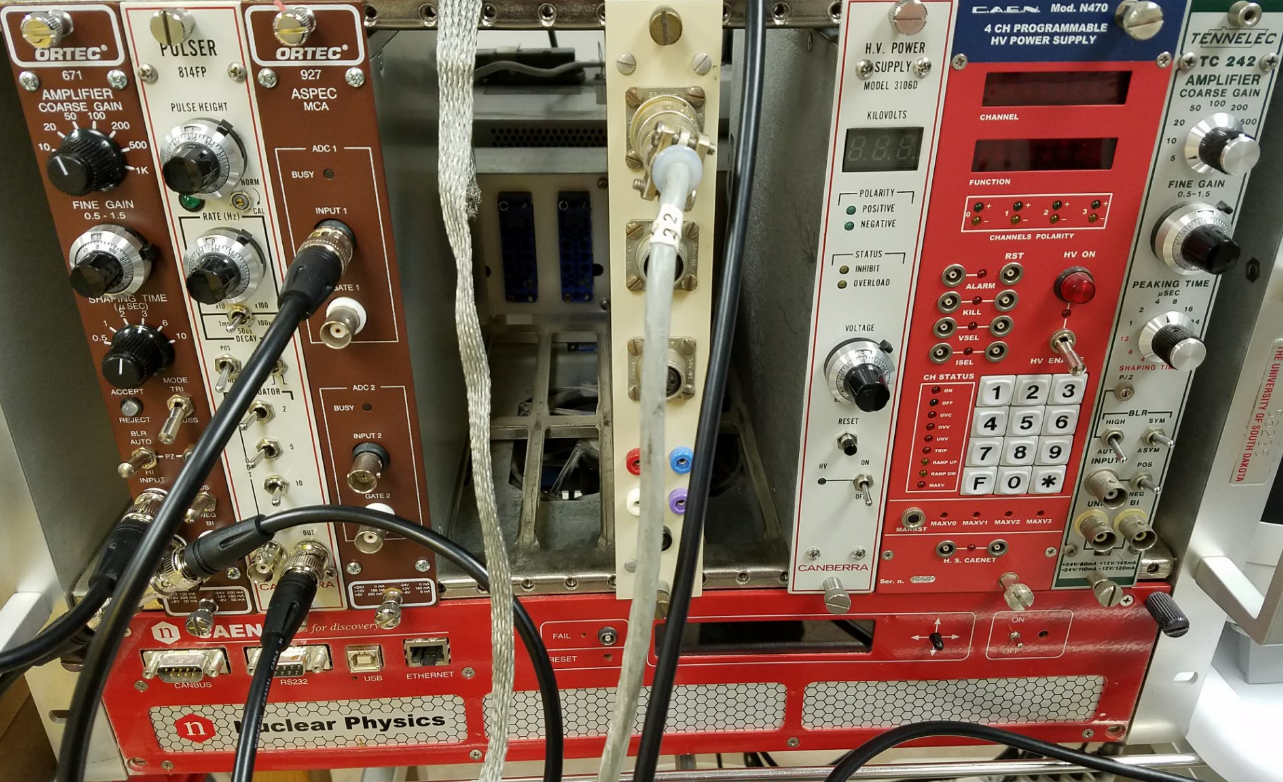
\includegraphics[width=\textwidth]{crate}
\caption{The electronics crate used in detector characterization}
\label{fig:crate}
\end{figure}

\begin{figure}[htpb]
\centering
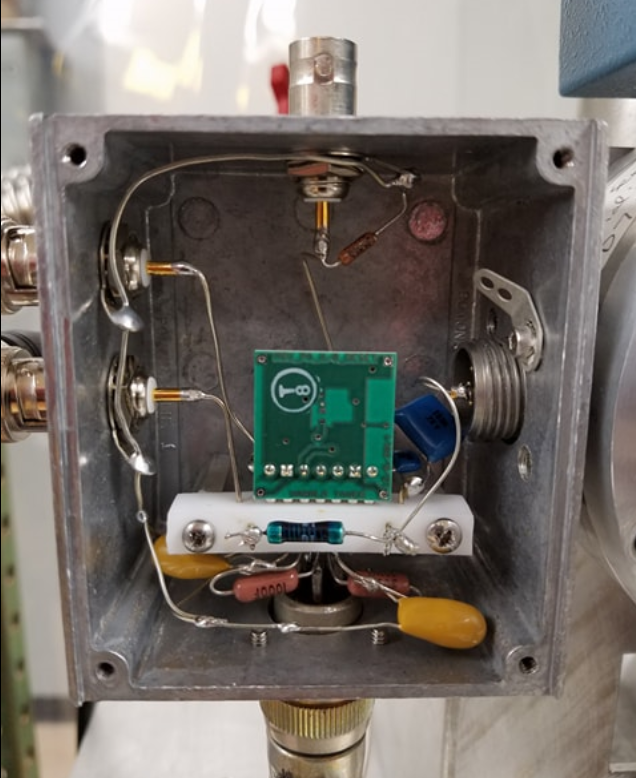
\includegraphics[width=0.7\textwidth]{left-ear}
\caption{Circuit box housing the preamplifier and leakage current assembly}
\label{fig:left-ear}
\end{figure}

\begin{figure}[htpb]
\centering
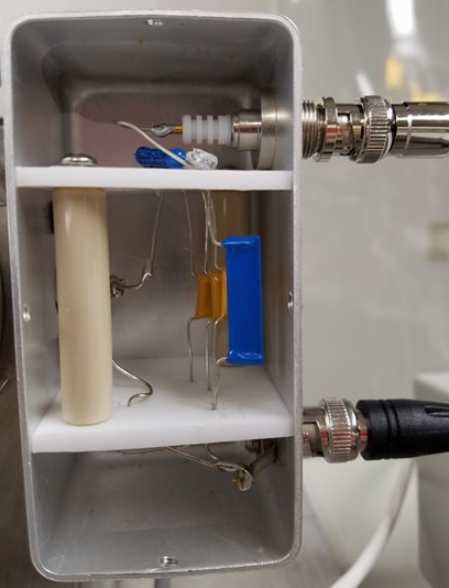
\includegraphics[width=0.7\textwidth]{right-ear}
\caption{Circuit box housing voltage and pulser input along with a high voltage filter}
\end{figure}

\begin{figure}[htpb]
\centering
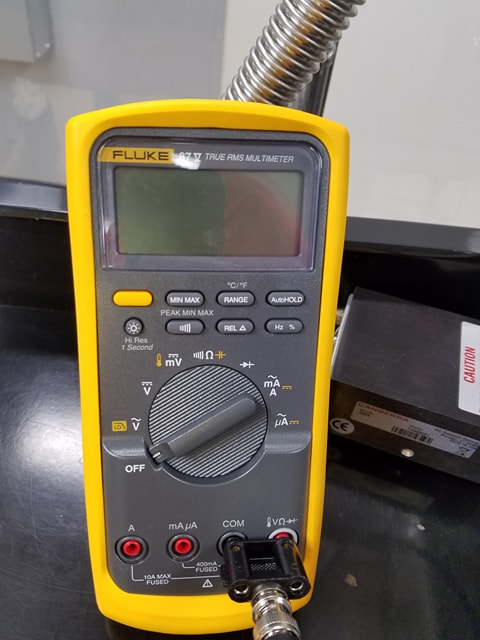
\includegraphics[width=0.7\textwidth]{multimeter}
\caption{Multimeter used to measure leakage current}
\label{fig:multimeter}
\end{figure}

\begin{figure}[htpb]
\centering
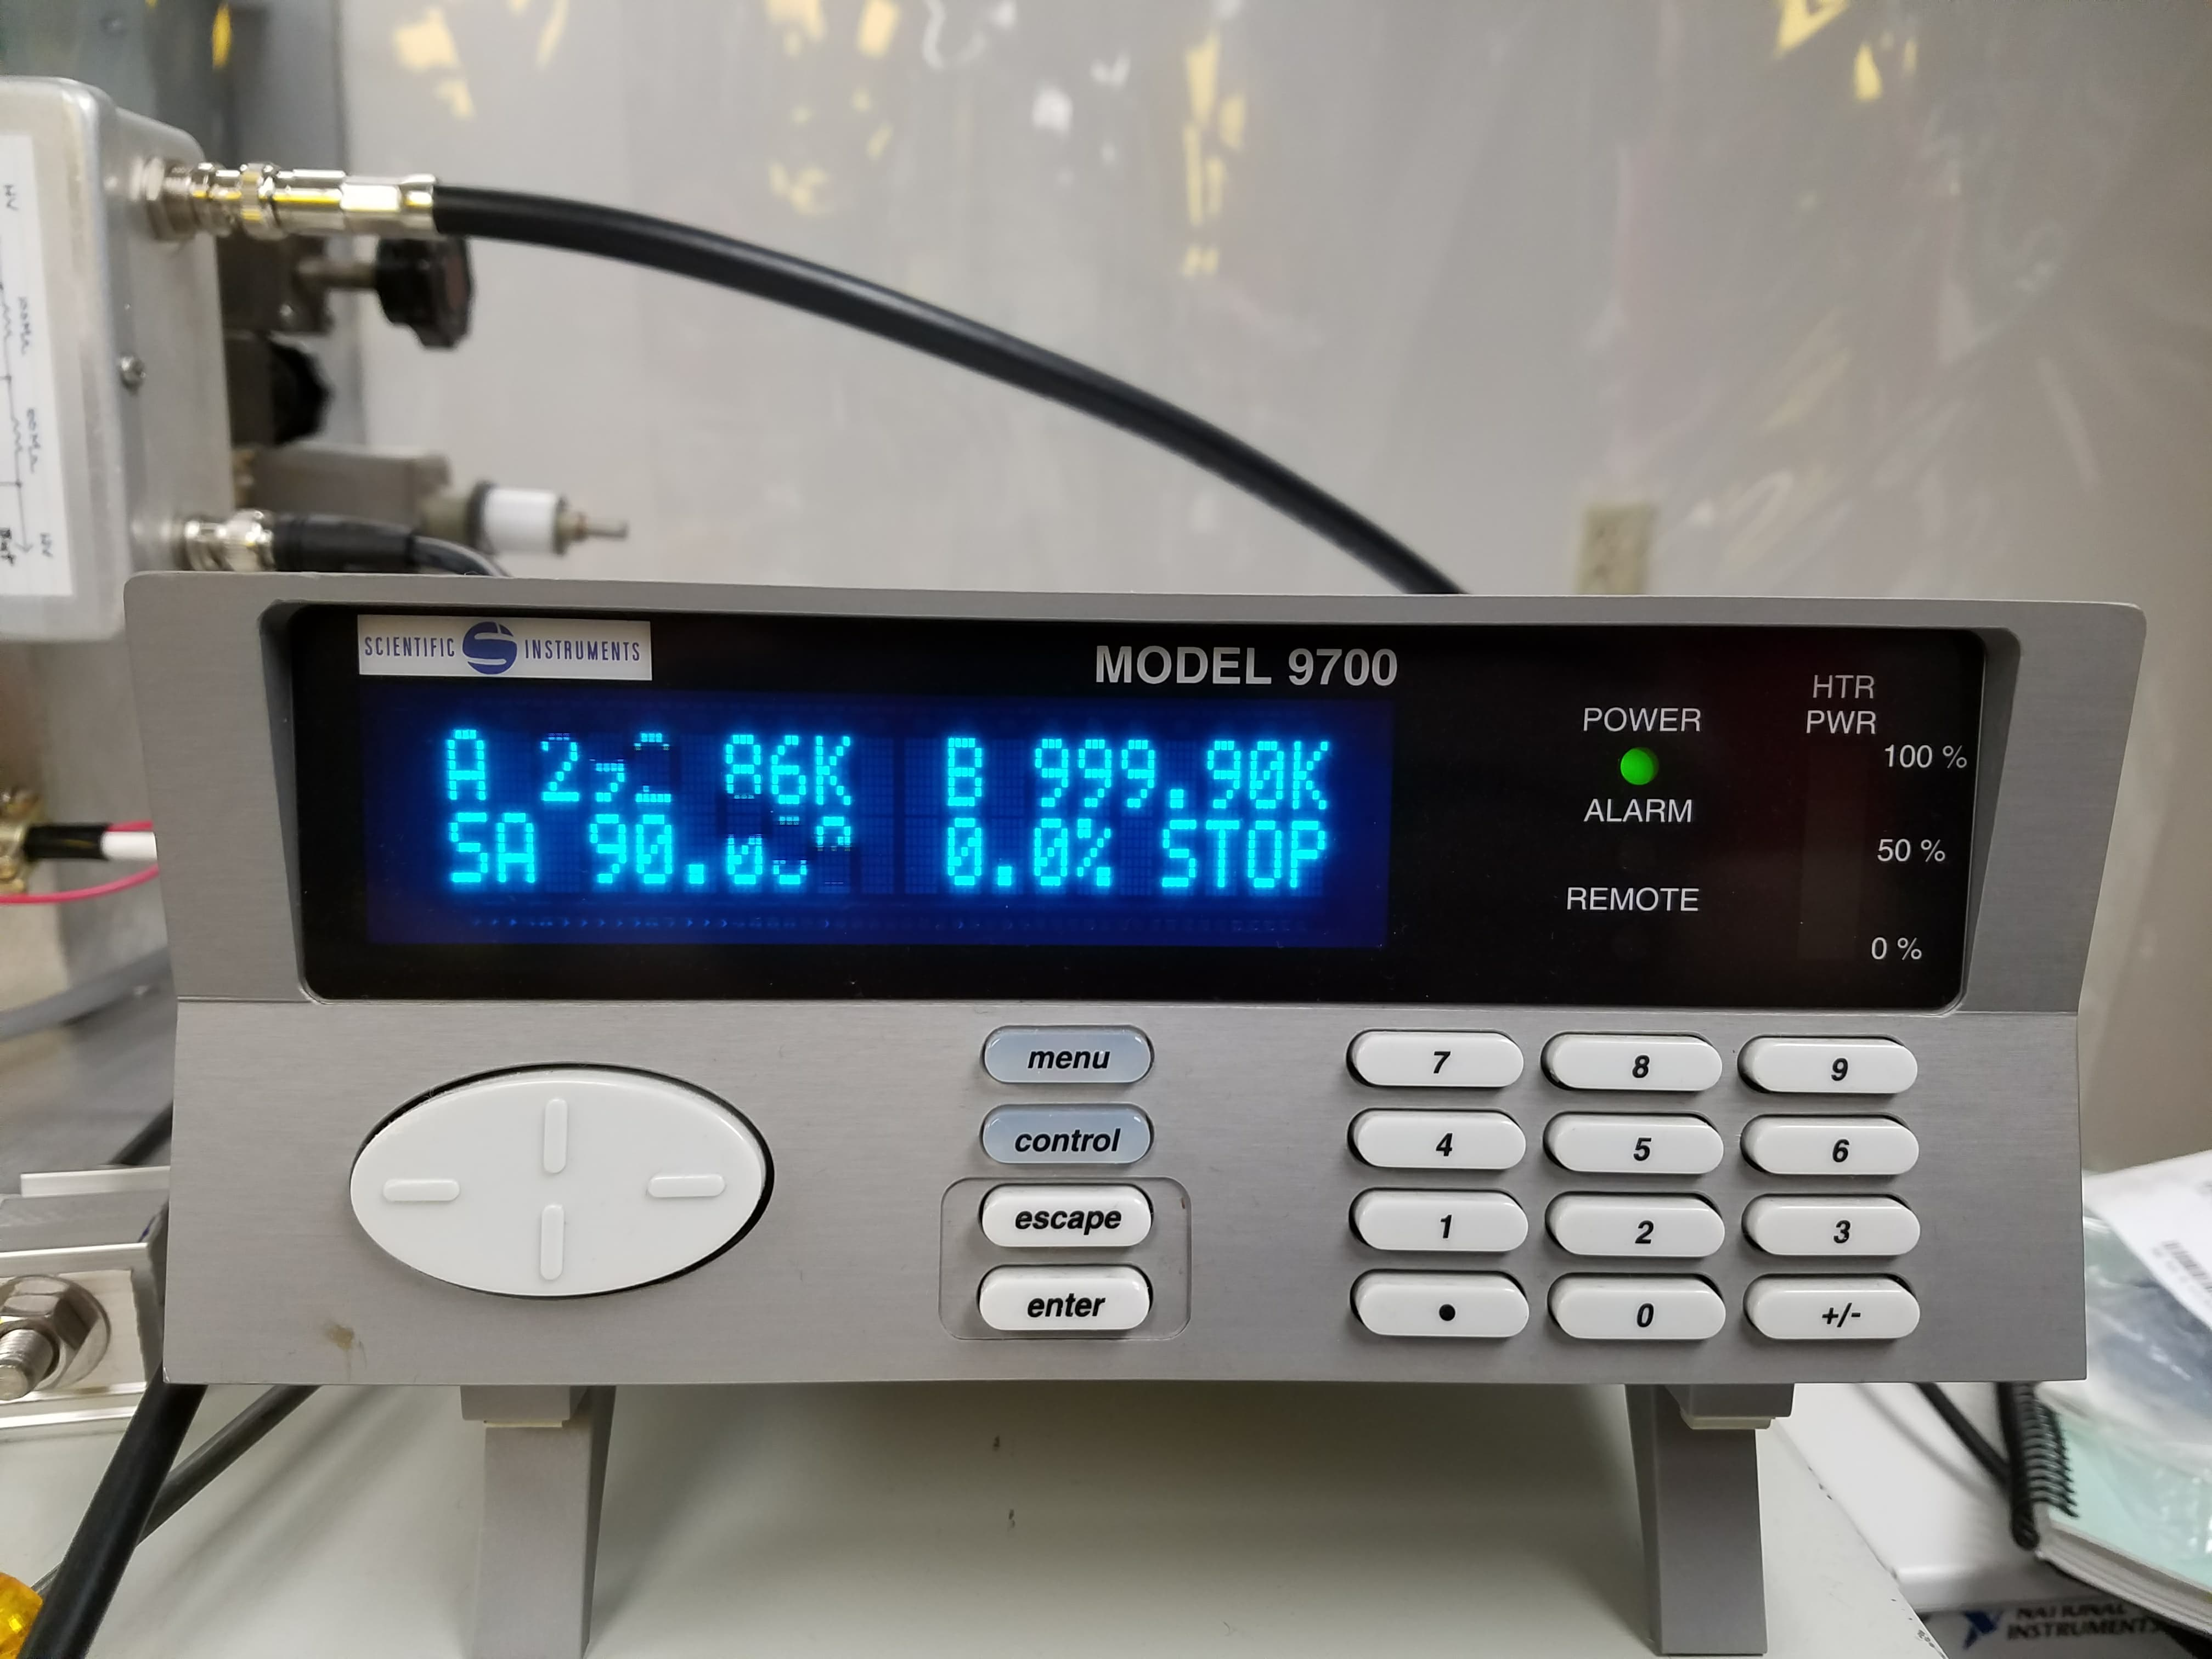
\includegraphics[width=\textwidth]{temp-sens}
\caption{Temperature monitoring and control system with heater}
\label{fig:temp-sens}
\end{figure}

\begin{figure}[htpb]
\centering
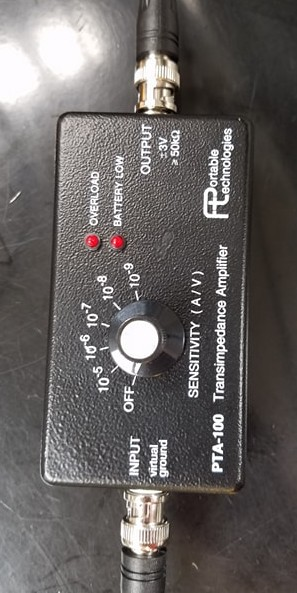
\includegraphics[width=0.5\textwidth]{transimpedence}
\caption{Device for converting low current to voltage}
\label{fig:transimpedence}
\end{figure}
